\begin{enumerate}[label=\thesubsection.\arabic*,ref=\thesubsection.\theenumi]
\item  Equal chords of a circle  are equidistant from the centre.
	\\
		\solution 
	In \figref{fig:ncert-circ-1},	
\begin{align}
	l &= 2r\sin \frac{\theta_1}{2}
	= 2r\sin \frac{\theta_2}{2}
	\\
	\implies \theta_1 &= \theta_2 = \theta
\end{align}
Thus, the distances
\begin{align}
	d_1 = r \cos \frac{\theta}{2} = d_2.
\end{align}
\begin{figure}[H]
	\begin{center}
		{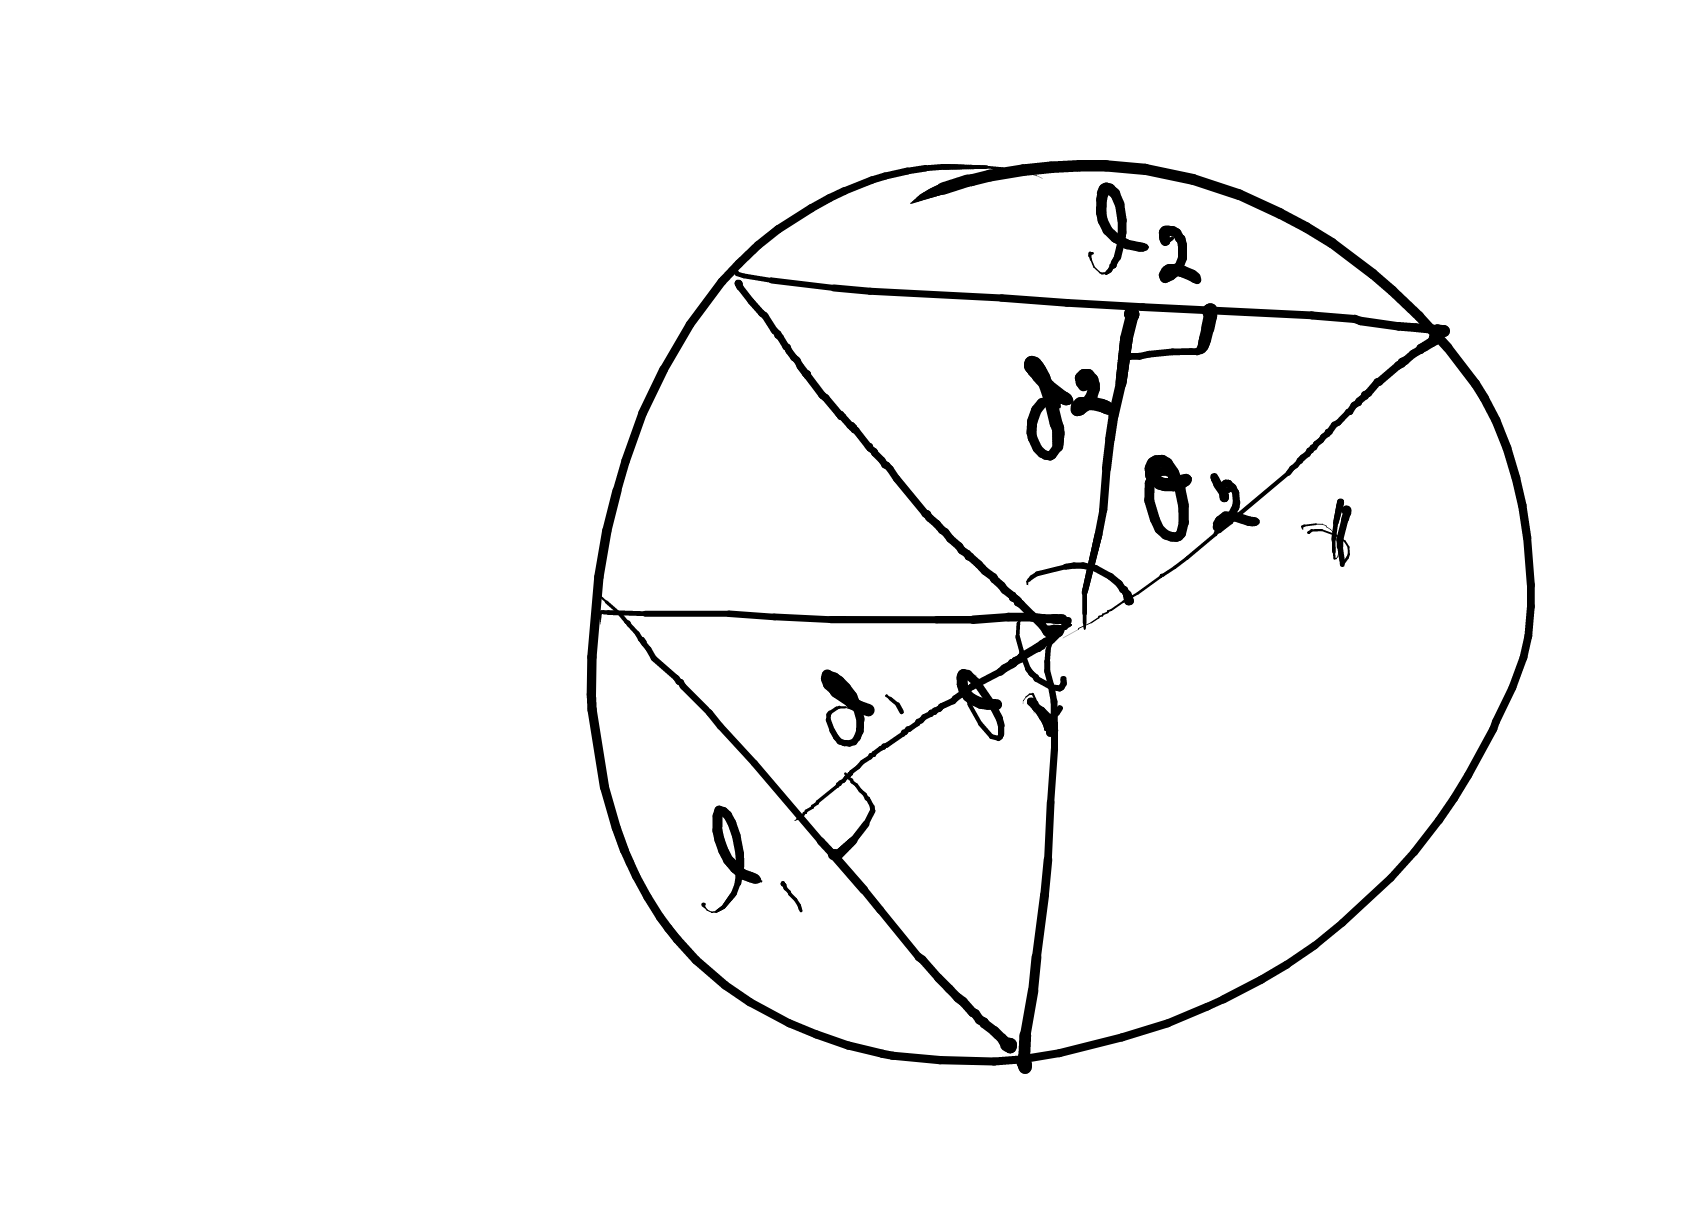
\includegraphics[width=0.6\columnwidth]{figs/ncert/circle/1.png}}
	\end{center}
	\caption{}
	\label{fig:ncert-circ-1}	
\end{figure}
%
\item Chords equidistant from the centre  of a circle  are equal.
\\
\solution
	In \figref{fig:ncert-circ-10}, 
\begin{align}
	l_1 = l_2 = 2d \tan \theta
\end{align}
\begin{figure}[H]
	\begin{center}
		{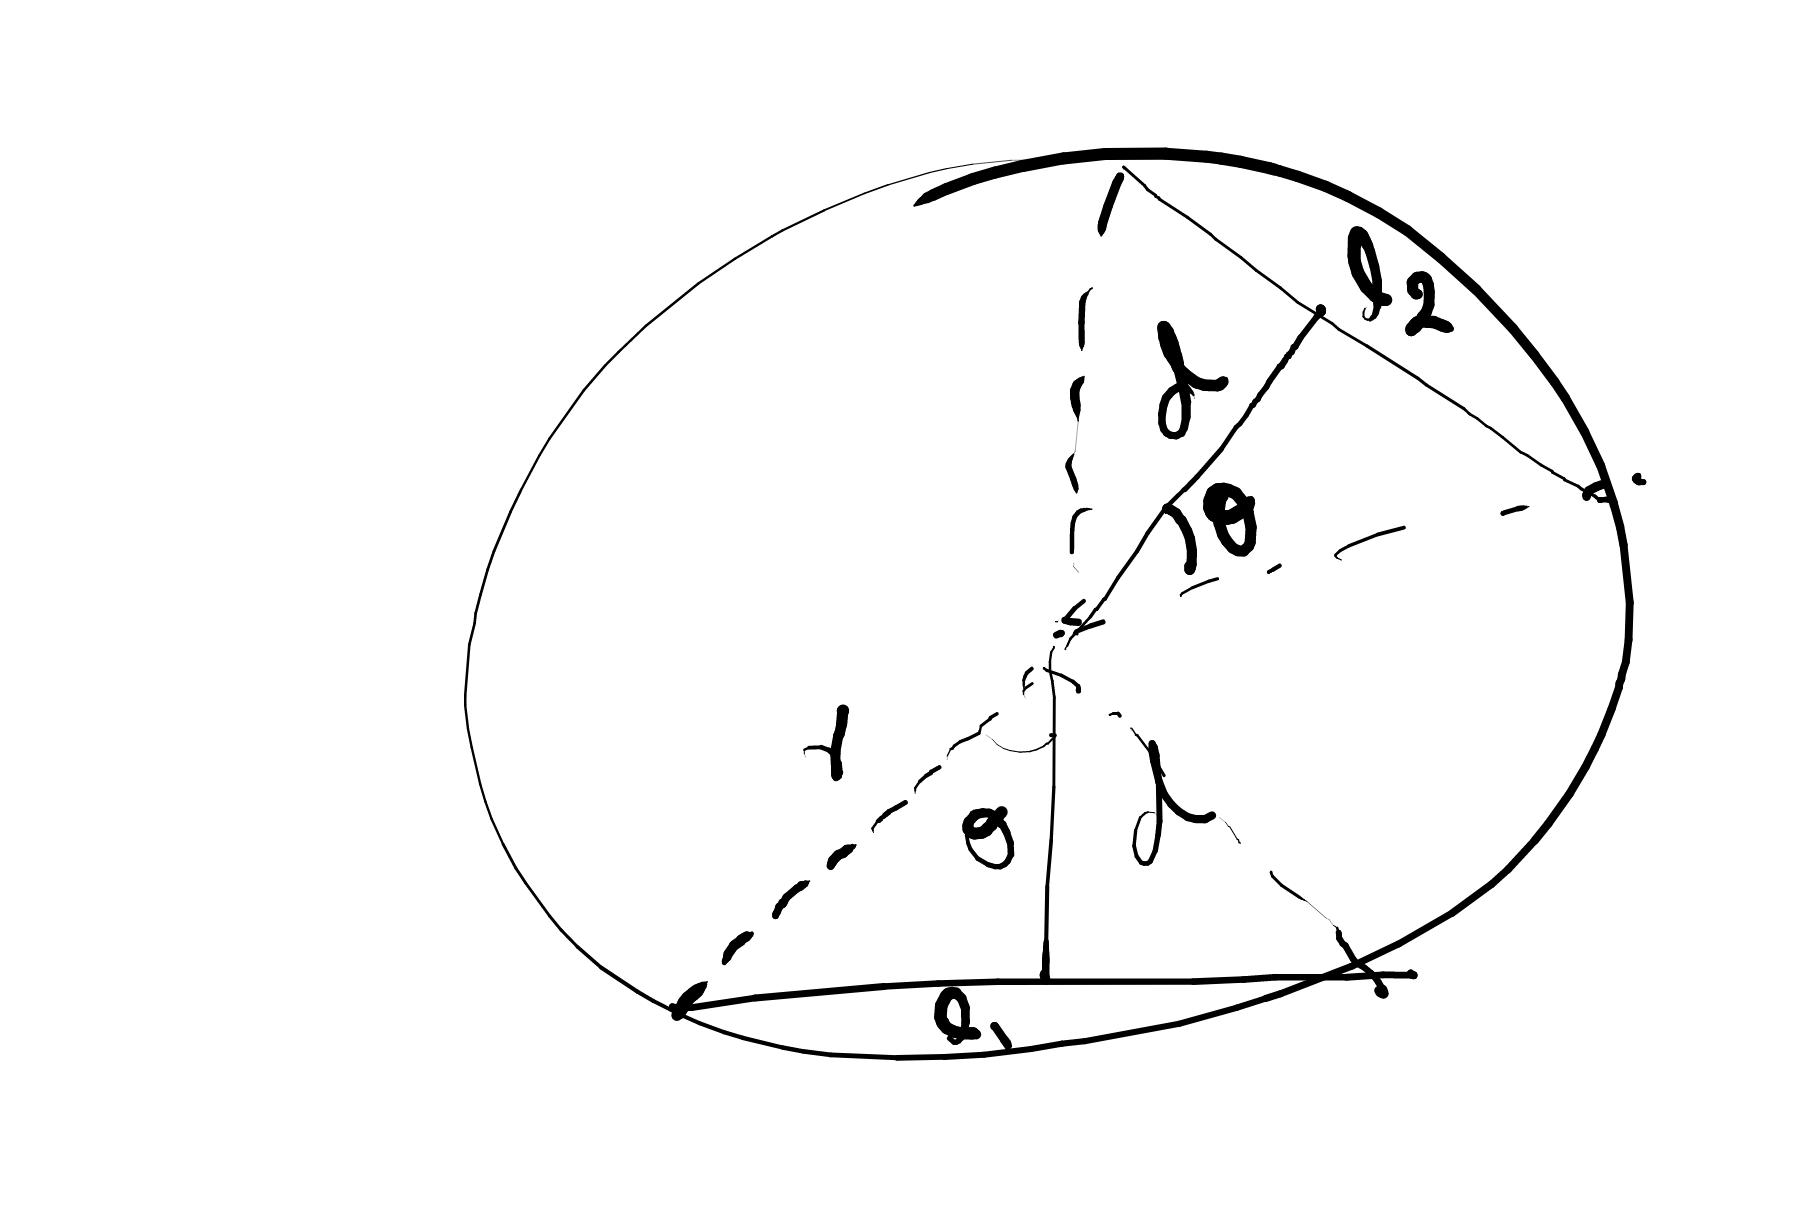
\includegraphics[width=0.6\columnwidth]{figs/ncert/circle/10.png}}
	\end{center}
	\caption{}
	\label{fig:ncert-circ-10}	
\end{figure}
%
 \item  Angle in a semicircle is a right angle. 
	\\
		\solution 
	In \figref{fig:ncert-circ-2}, considering a unit circle	
	with
\begin{align}
	\vec{A}&= \myvec{\cos \theta \\ \sin \theta}\,
	\vec{B}= \myvec{-1 \\ 0}\,
	\vec{C}= \myvec{1 \\ 0}
	\\
	\brak{A-B}^{\top}
	\brak{A-C}^{\top}
	&=
	 \myvec{\cos \theta+1 & \sin \theta}
\myvec{\cos \theta -1 \\ \sin \theta}
\\
	&=\cos^2\theta -1 + \sin^2\theta = 0
\end{align}
Thus, $AB \perp AC$.
\begin{figure}[H]
	\begin{center}
		{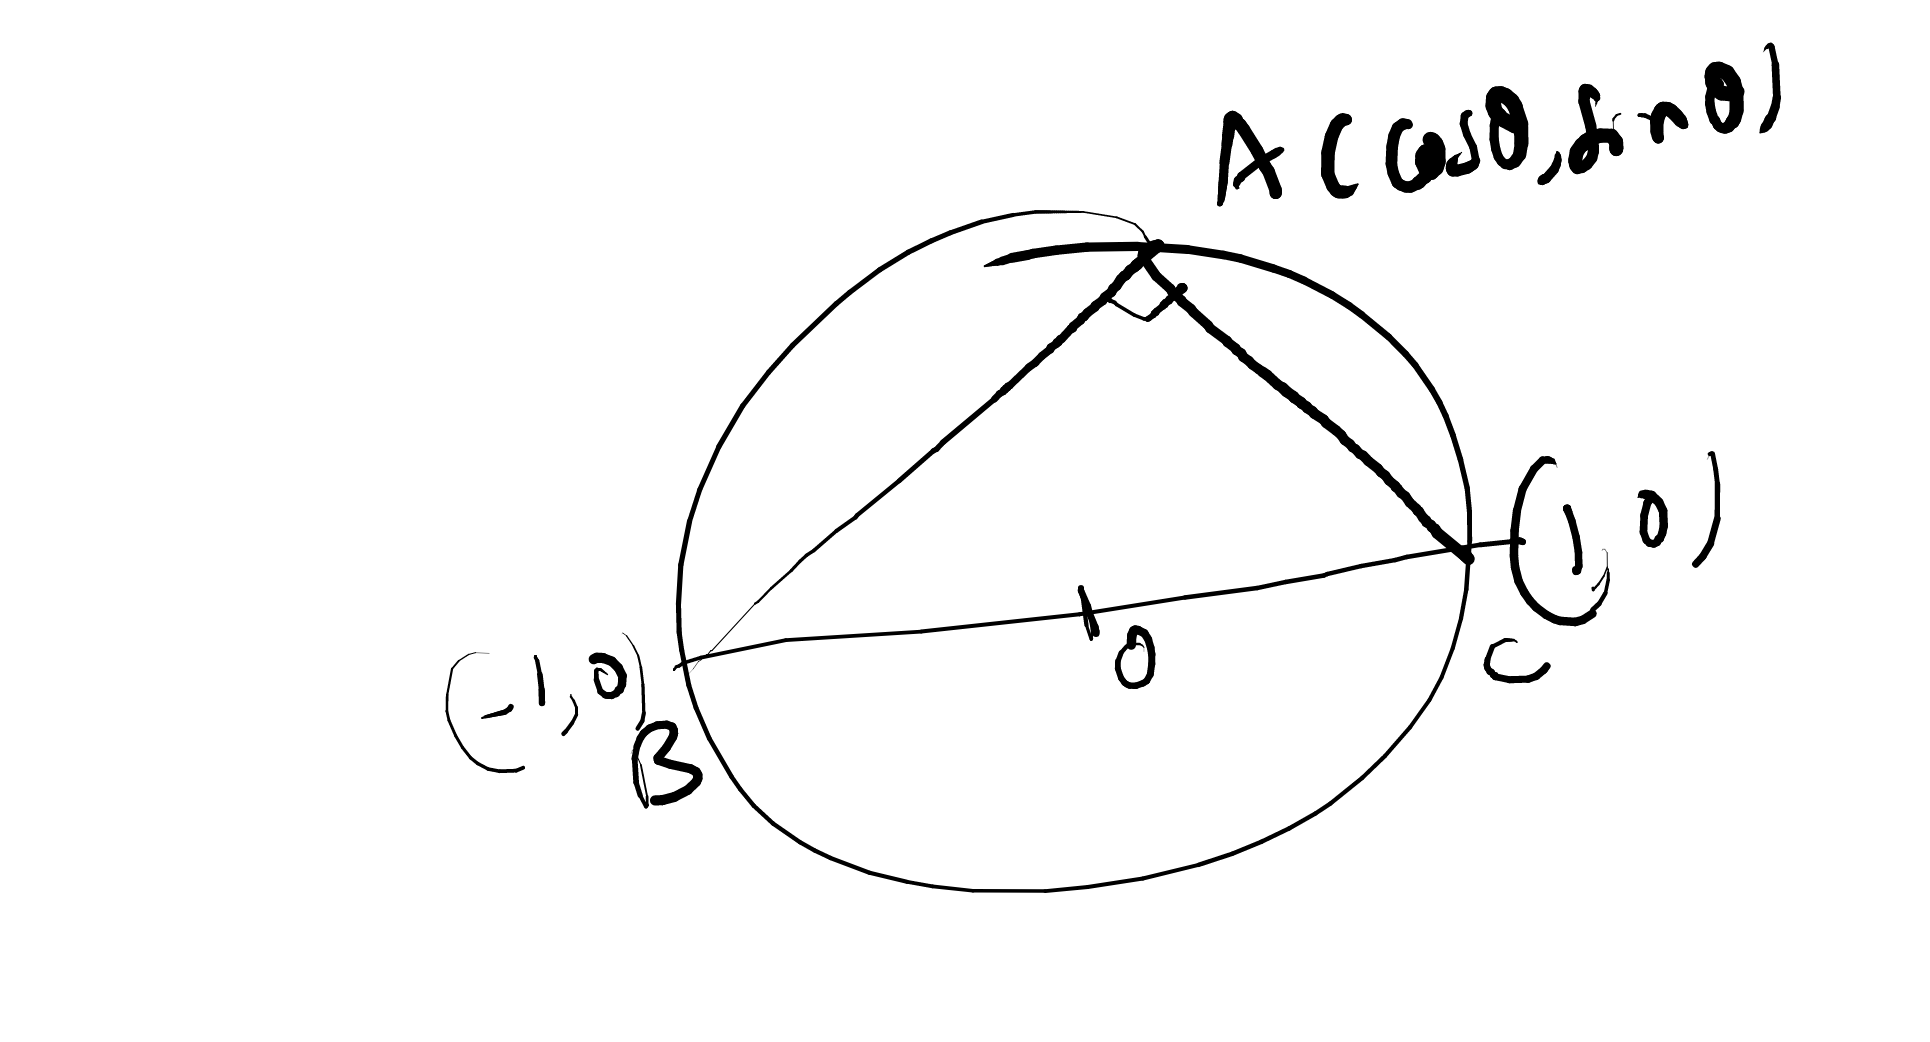
\includegraphics[width=0.6\columnwidth]{figs/ncert/circle/2.png}}
	\end{center}
	\caption{}
	\label{fig:ncert-circ-2}	
\end{figure}
%
%
\item Two circles of radii 5 cm and 3 cm intersect at two points and the distance between their centres is 4 cm. Find the length of the common chord.
	\\
		\solution 
	In \figref{fig:ncert-circ-3}, 
\begin{align}
	\cos \alpha &= \frac{r_1^2+d^2-r_2^2}{2r_1r_2} = 0.8
	\\
\implies	l &= 2r_1\sin \alpha = 6
\end{align}
upon substituting numerical values.
\begin{figure}[H]
	\begin{center}
		{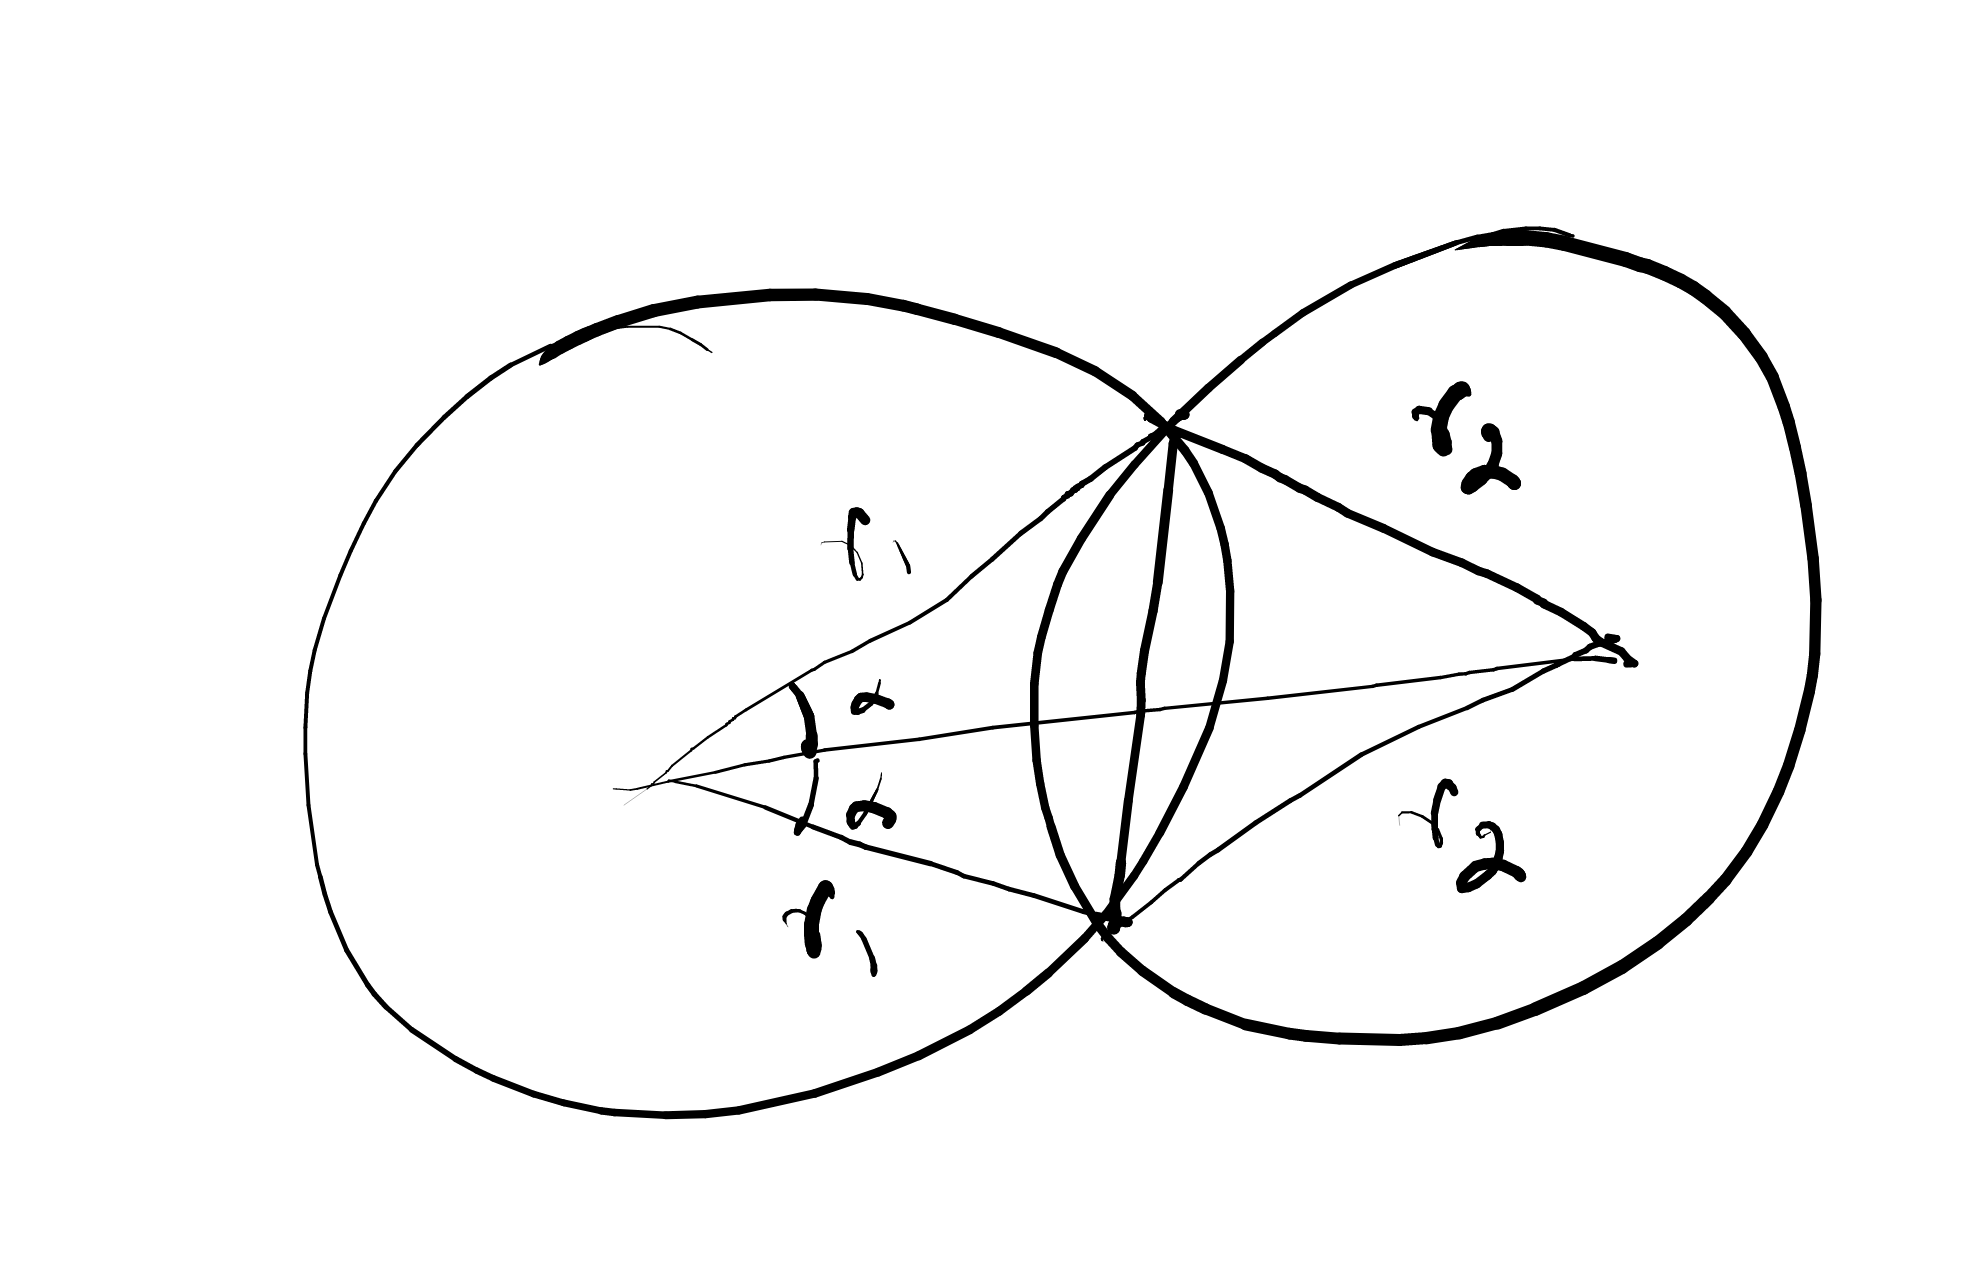
\includegraphics[width=0.6\columnwidth]{figs/ncert/circle/3.png}}
	\end{center}
	\caption{}
	\label{fig:ncert-circ-3}	
\end{figure}
%
\item Two chords $AB$ and $CD$ of lengths 5 cm and 11 cm respectively of a circle are parallel
to each other and are on opposite sides of its centre. If the distance between $AB$ and
$CD$ is 6 cm, find the radius of the circle.
	\\
		\solution 
	In \figref{fig:ncert-circ-4}, 
\begin{align}
	l_1&=2r \sin \theta_1\,
	l_2=2r \sin \theta_2
	\\
	d &= r \brak{\cos \theta_1+\cos \theta_2}
\end{align}
yielding
\begin{align}
	2d &=  \sqrt{4r^2-l_1^2}+\sqrt{4r^2-l_2^2}
	\\
	\implies 
	\brak{2d -  \sqrt{4r^2-l_1^2}}^2&=4r^2-l_2^2
	\\
	\text{or, }4d^2 -l_1^2+l_2^2&=4d\sqrt{4r^2-l_1^2}
	\\
	\implies r &= \frac{\sqrt{\brak{\frac{4d^2 -l_1^2+l_2^2}{4d}}^2+l_1^2}}{2} = 5.59 
\end{align}
upon substituting numerical values.
\begin{figure}[H]
	\begin{center}
		{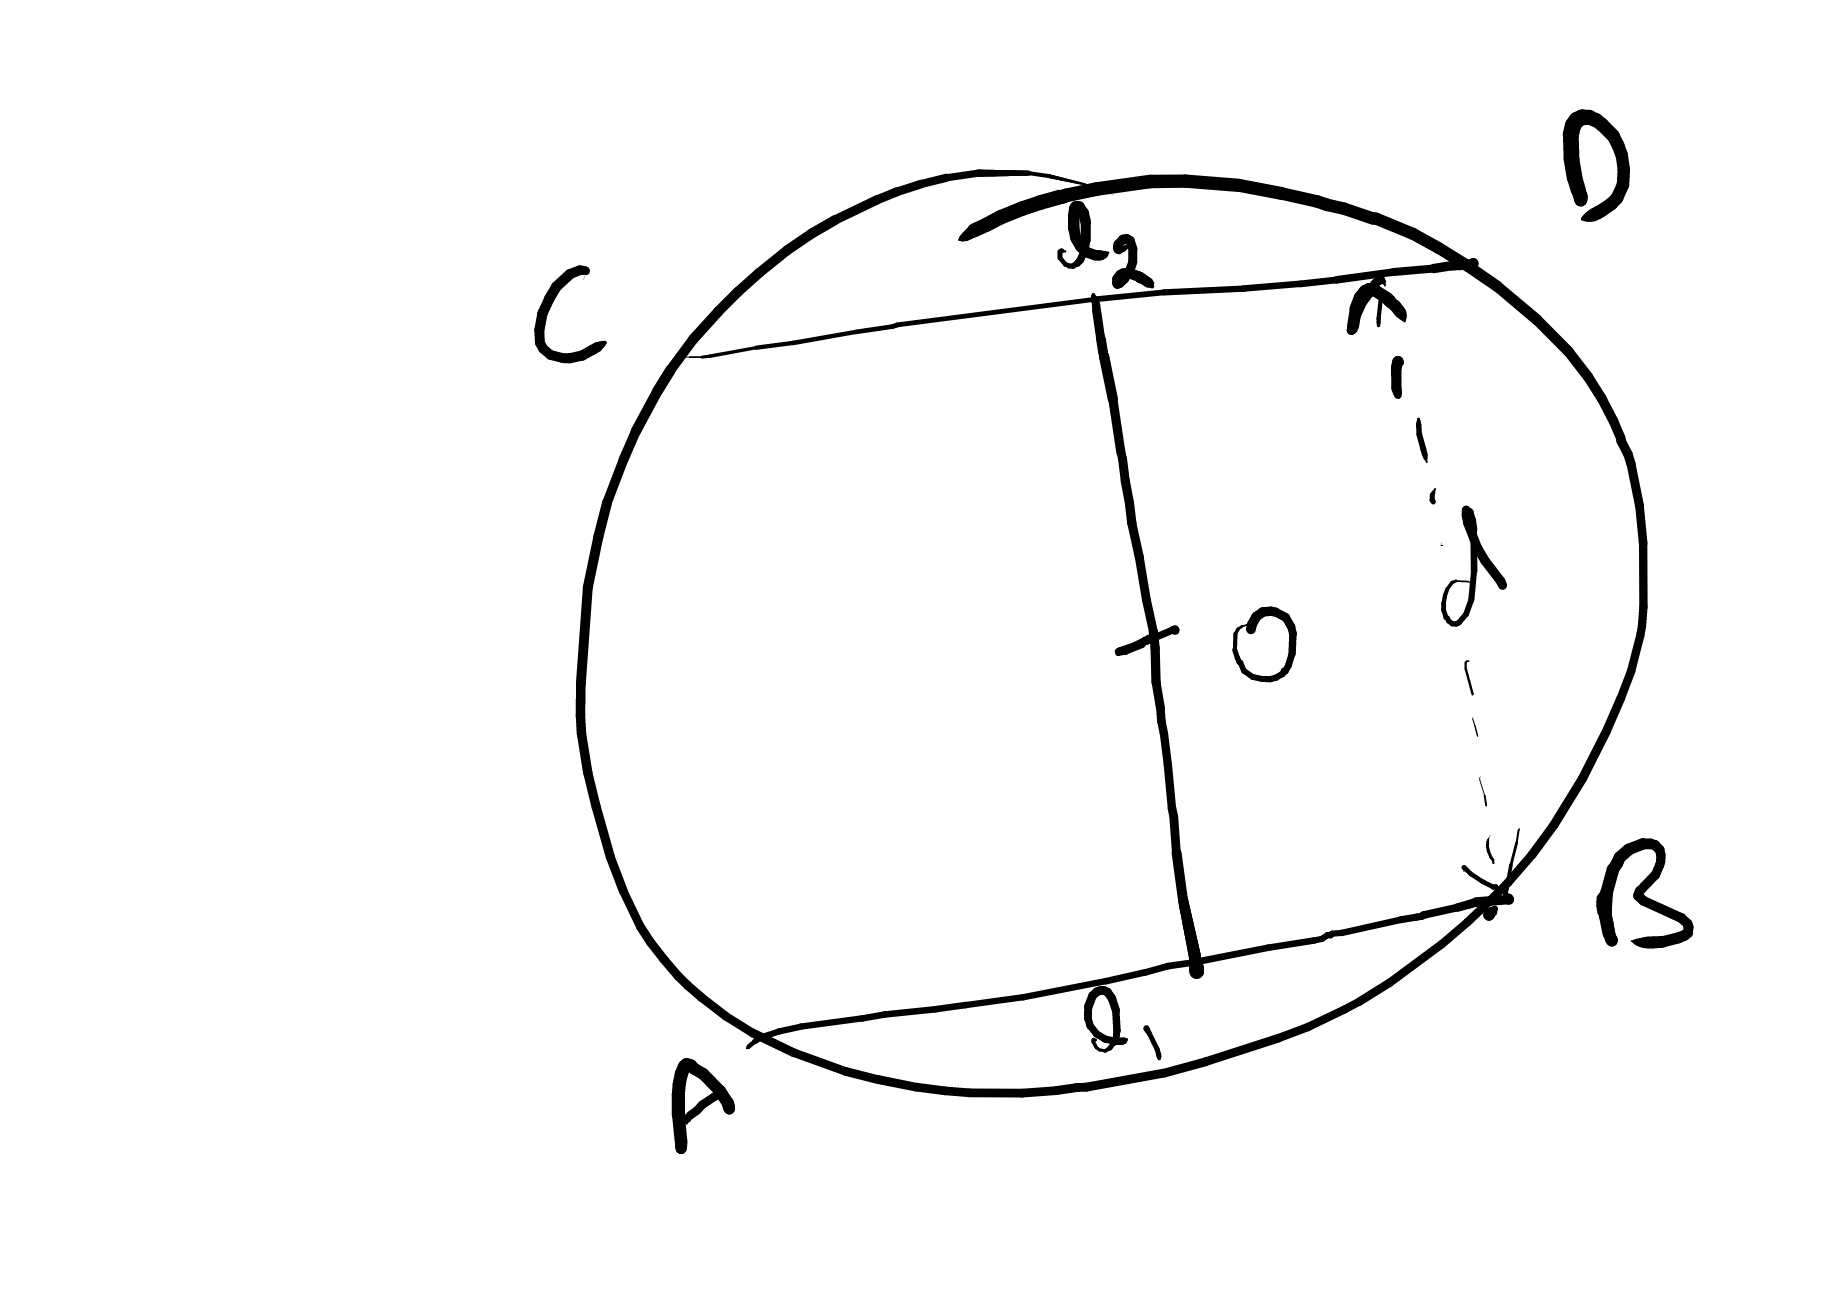
\includegraphics[width=0.6\columnwidth]{figs/ncert/circle/4.png}}
	\end{center}
	\caption{}
	\label{fig:ncert-circ-4}	
\end{figure}
%
\item The lengths of two parallel chords of a circle are 6 cm and 8 cm. If the smaller chord is
at distance 4 cm from the centre, what is the distance of the other chord from the
centre?
\\
\solution
	In \figref{fig:ncert-circ-5}, 
\begin{align}
	l_1&=2r \sin \theta_1\,
	l_2=2r \sin \theta_2
	\\
	d_1 &= r \cos \theta_1\,
	d_2 =r\cos \theta_2
\end{align}
yielding
\begin{align}
	\theta_1 &= \tan^{-1}\brak{\frac{l_1}{2d_1}}
	\\
	\theta_2 &= \sin^{-1}\brak{\frac{l_2\cos \theta_1}{2d_1}}	
	\\
	\implies d_2 &= \frac{l_2}{2}\cot\theta_2 = 3
\end{align}
upon substituting numerical values.
\begin{figure}[H]
	\begin{center}
		{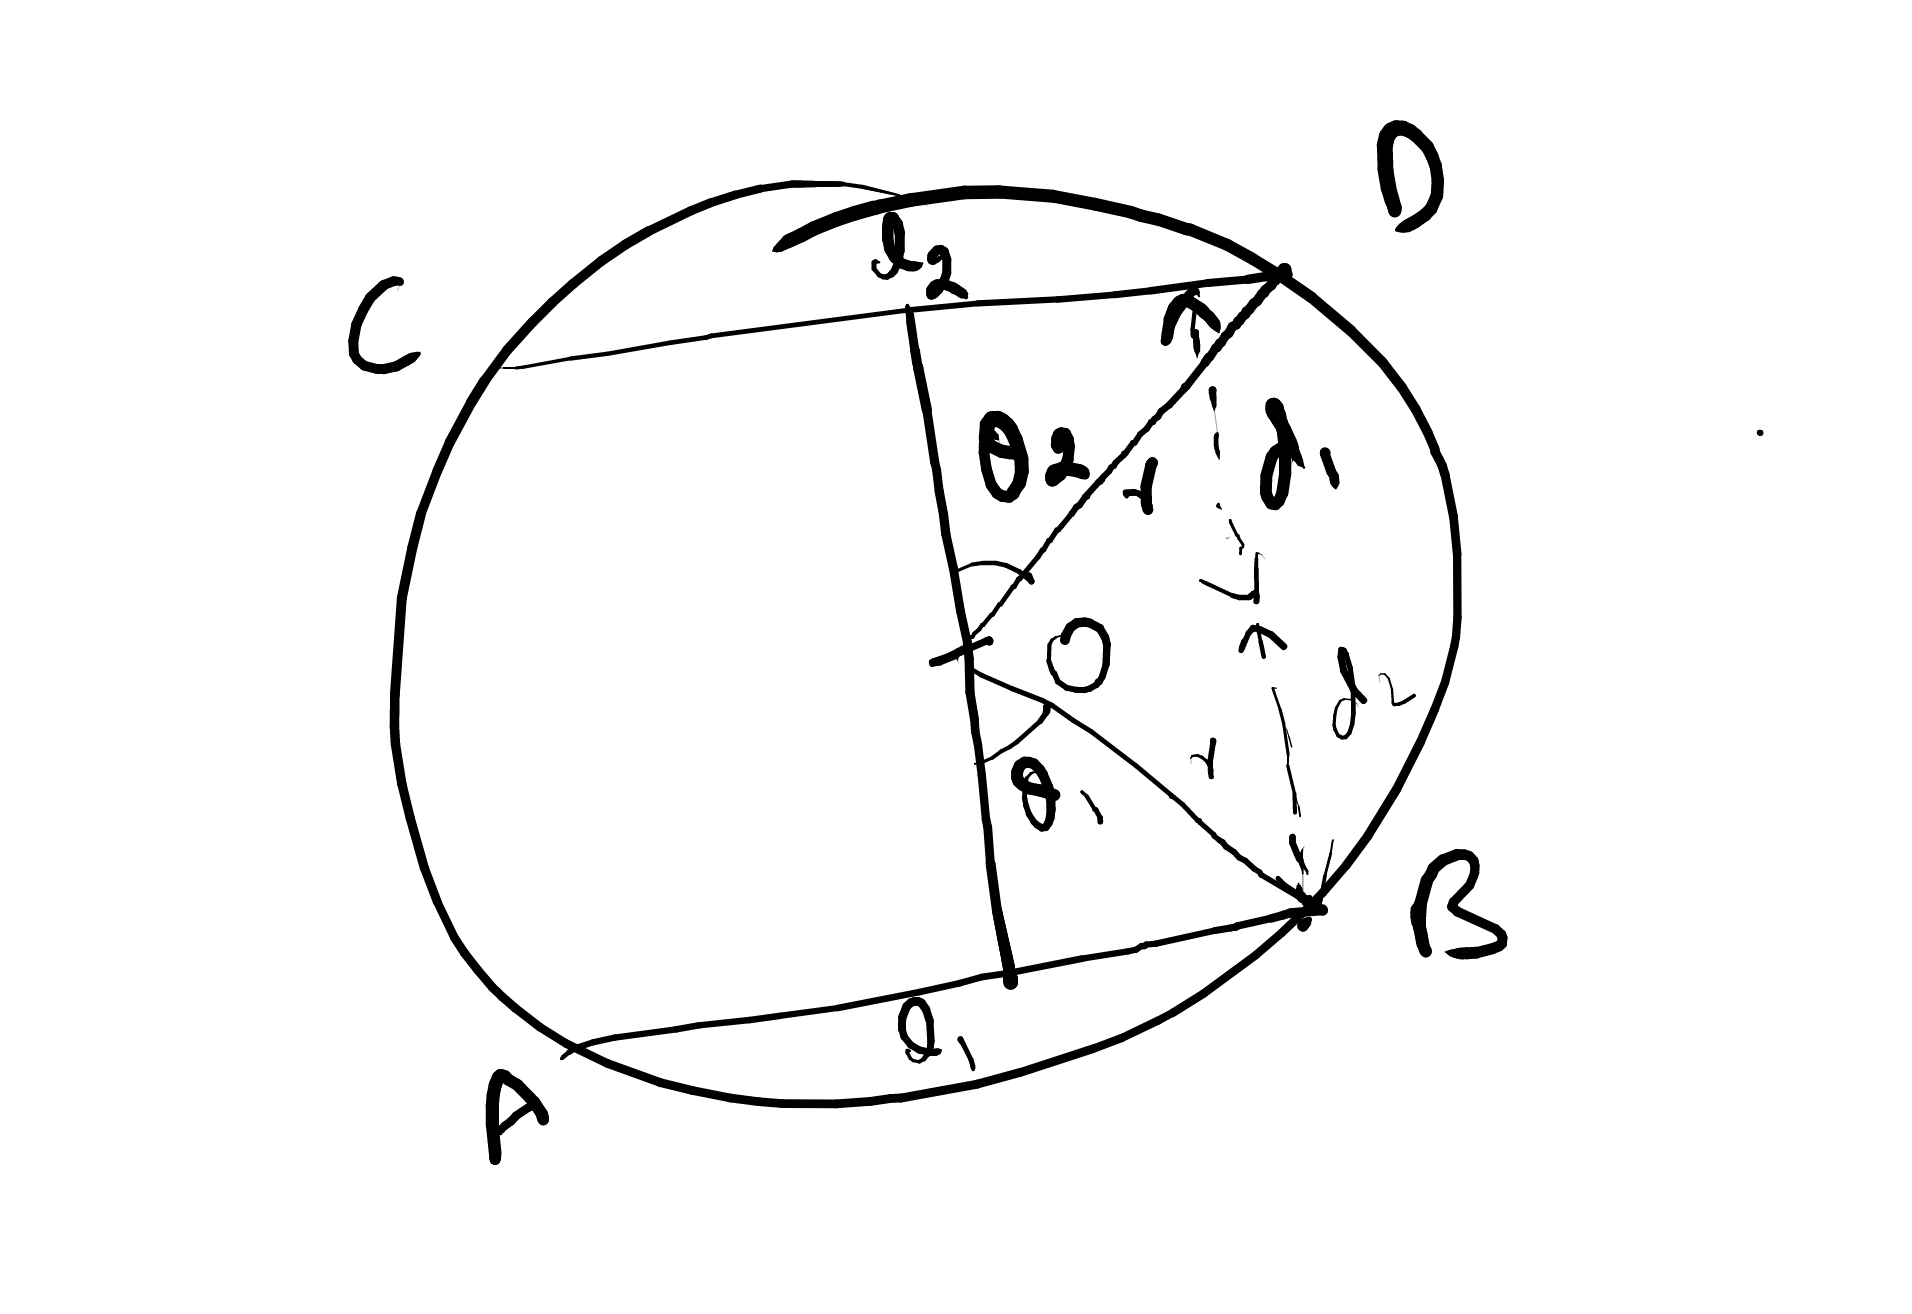
\includegraphics[width=0.6\columnwidth]{figs/ncert/circle/5.png}}
	\end{center}
	\caption{}
	\label{fig:ncert-circ-5}	
\end{figure}
%
\item  Two concentric circles are of radii 5 cm and 3 cm. Find the length of the chord of the larger circle which touches the smaller circle.
\\
\solution
	In \figref{fig:ncert-circ-6}, 
\begin{align}
	\theta &= \cos^{-1}\brak{\frac{r_2}{r_1}}
	\\
\implies	l &= 2r_1\sin \theta = 8
\end{align}
upon substituting numerical values.
\begin{figure}[H]
	\begin{center}
		{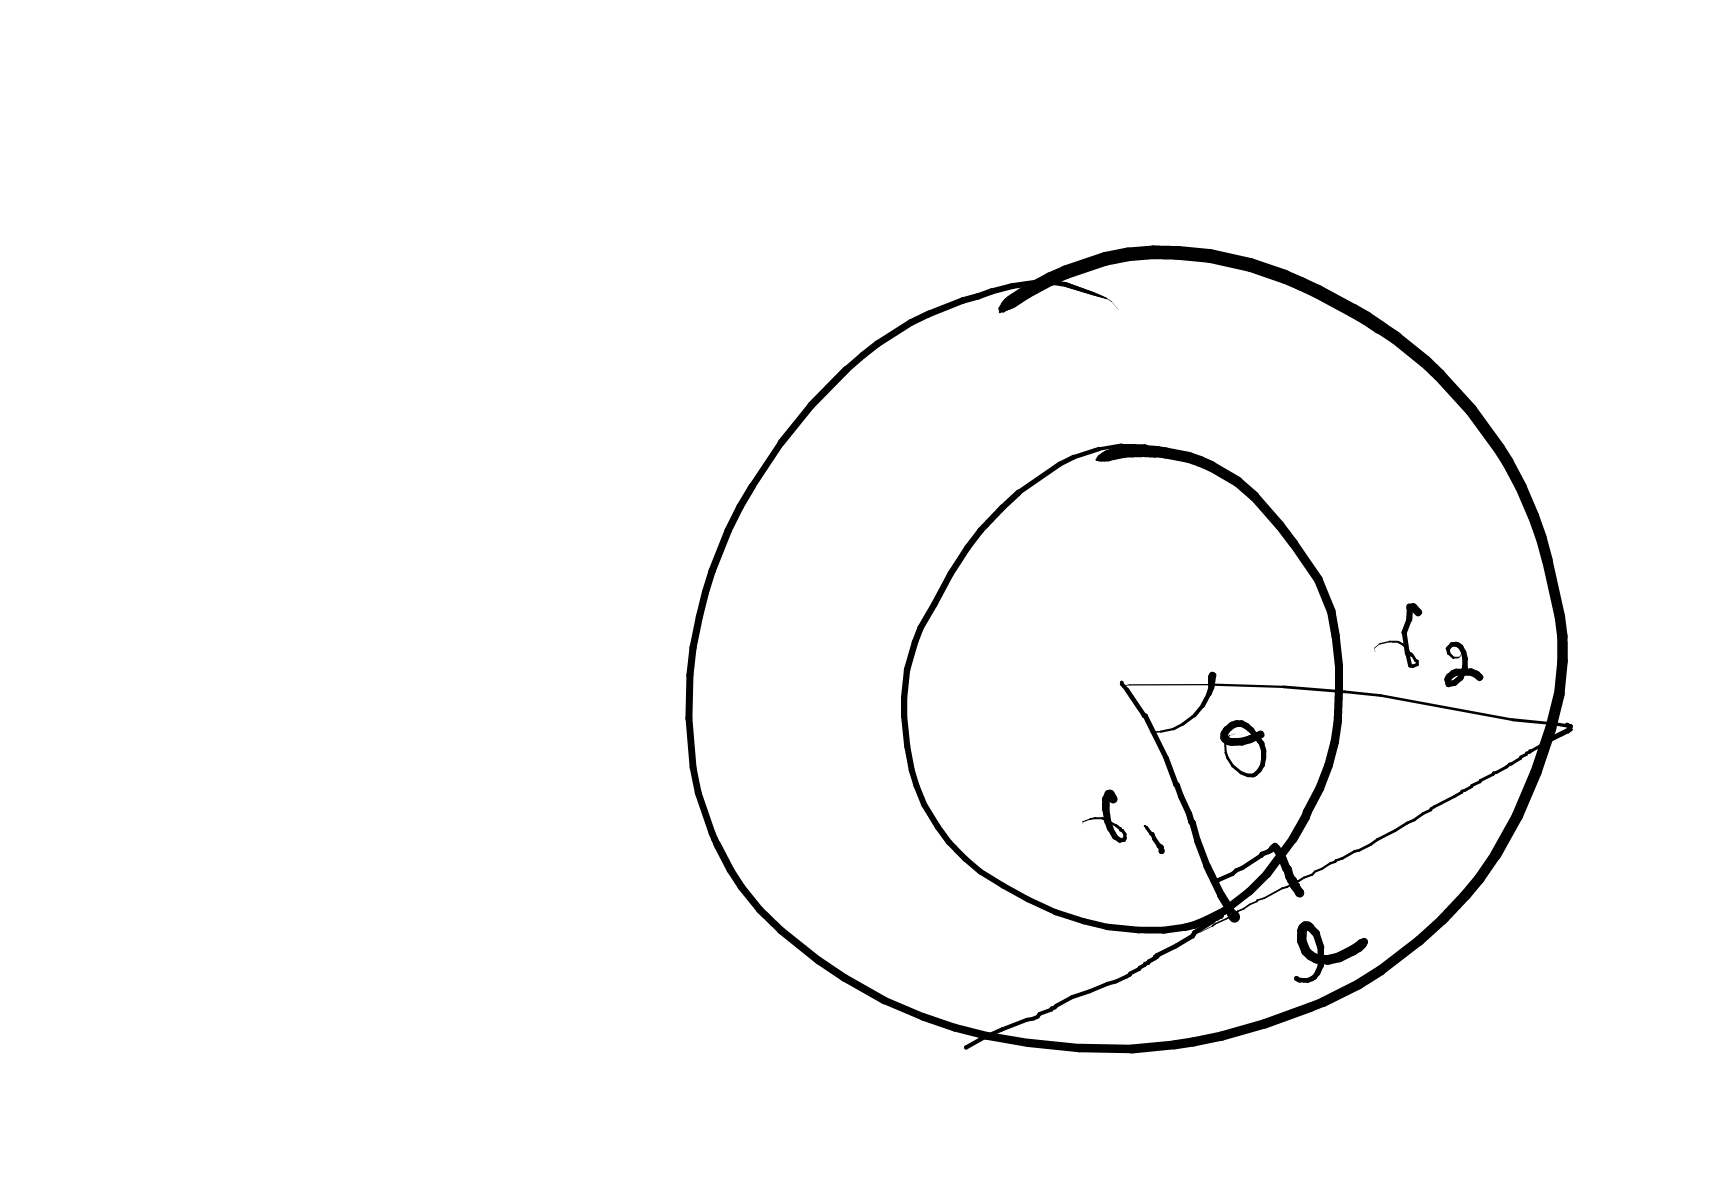
\includegraphics[width=0.6\columnwidth]{figs/ncert/circle/6.png}}
	\end{center}
	\caption{}
	\label{fig:ncert-circ-6}	
\end{figure}
%
\item A $\triangle ABC$ is drawn to circumscribe a circle of radius 4 cm such that the segments $BD$ and $DC$ into which $BC$ is divided by the point of contact $D$ are of lengths 8 cm and 6 cm respectively. Find the sides $AB$ and $AC$.
\\
\solution
	In \figref{fig:ncert-circ-7}, 
\begin{align}
	a &= a_1+a_2
	\\
	\frac{B}{2} &= \tan^{-1}\frac{r}{a_1}
	\\
	\implies B &= 2\tan^{-1}\frac{r}{a_1}
	\\
	\frac{C}{2} &= \tan^{-1}\frac{r}{a_2}
	\\
	\implies C &= 2\tan^{-1}\frac{r}{a_2}
	\\
	\text{and } A = \pi - B-C
\end{align}
Using sine formula,
\begin{align}
	b &= a\frac{\sin B}{\sin A}=13
	\\
	c &= a\frac{\sin C}{\sin A}=15
\end{align}
\begin{figure}[H]
	\begin{center}
		{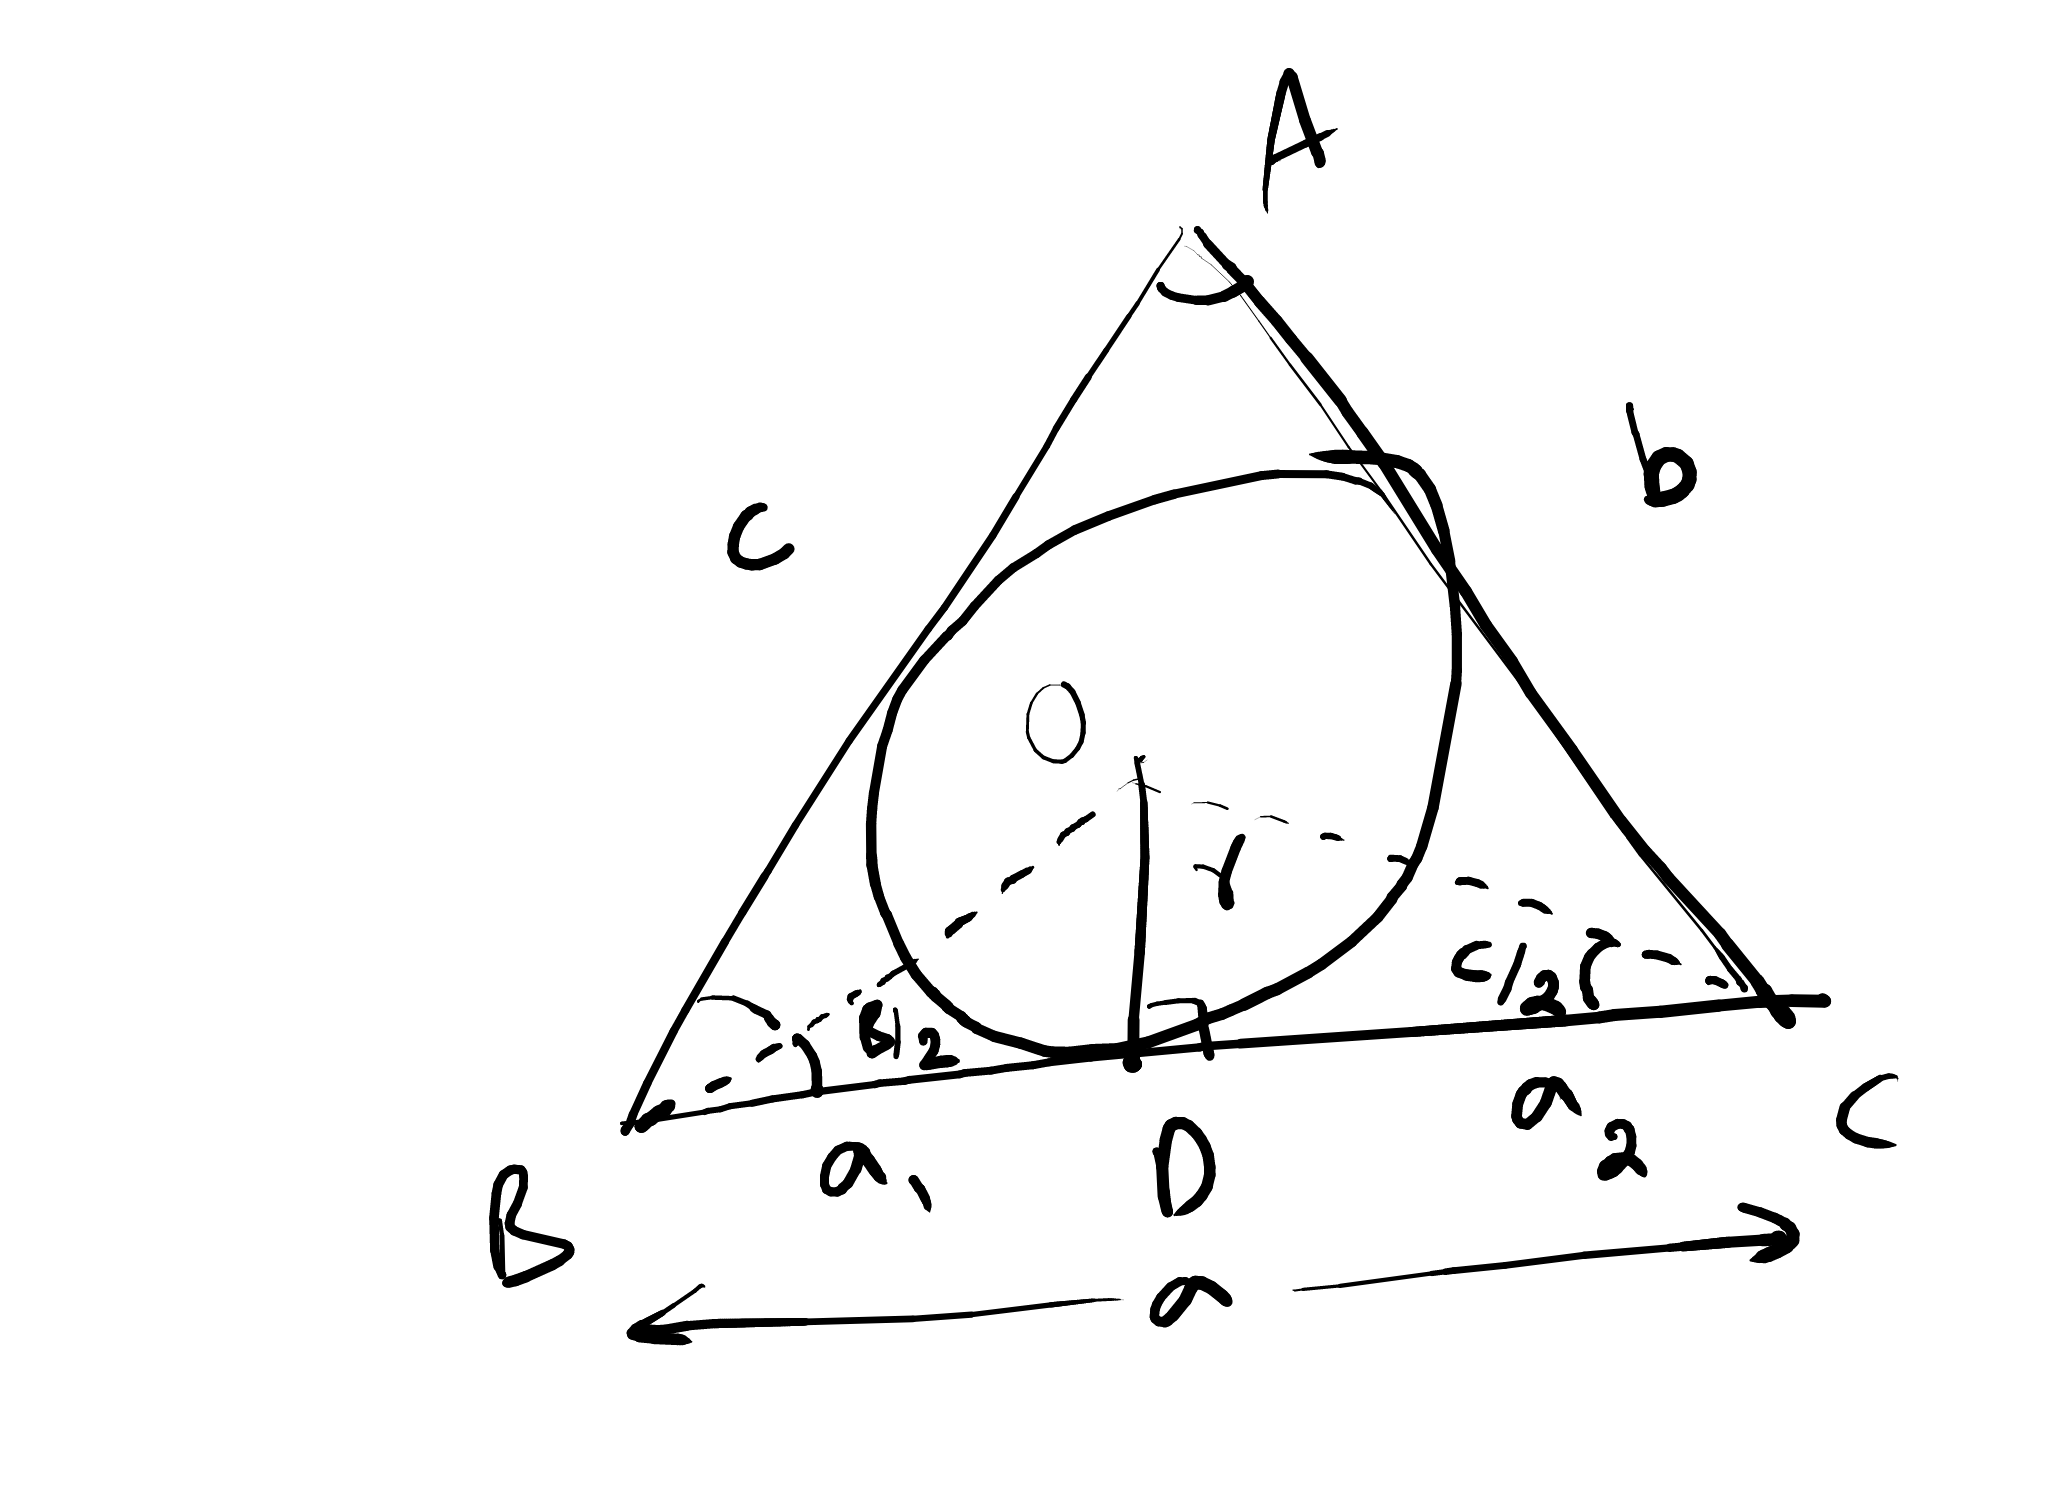
\includegraphics[width=0.6\columnwidth]{figs/ncert/circle/7.png}}
	\end{center}
	\caption{}
	\label{fig:ncert-circ-7}	
\end{figure}
\item $PQ$ is a chord of length 8 cm of a circle of radius 5 cm. The tangents at $P$ and $Q$ intersect at a point $T$. Find the length $TP$.
\\
\solution
	In \figref{fig:ncert-circ-8}, 
\begin{align}
	\frac{\theta}{2} &= \sin^{-1}\frac{l}{2r}
	\\
	\implies \theta &= 2\sin^{-1}\frac{l}{2r}
	\\
	\text{and }T &= \pi - \theta
\end{align}
Also, 
\begin{align}
	l &= 2x \sin \frac{T}{2} = 2x \cos \frac{\theta}{2}
	\\
	 \implies x &= \frac{l}{2} \sec\frac{\theta}{2}=6.67
\end{align}
upon substituting numerical values.
\begin{figure}[H]
	\begin{center}
		{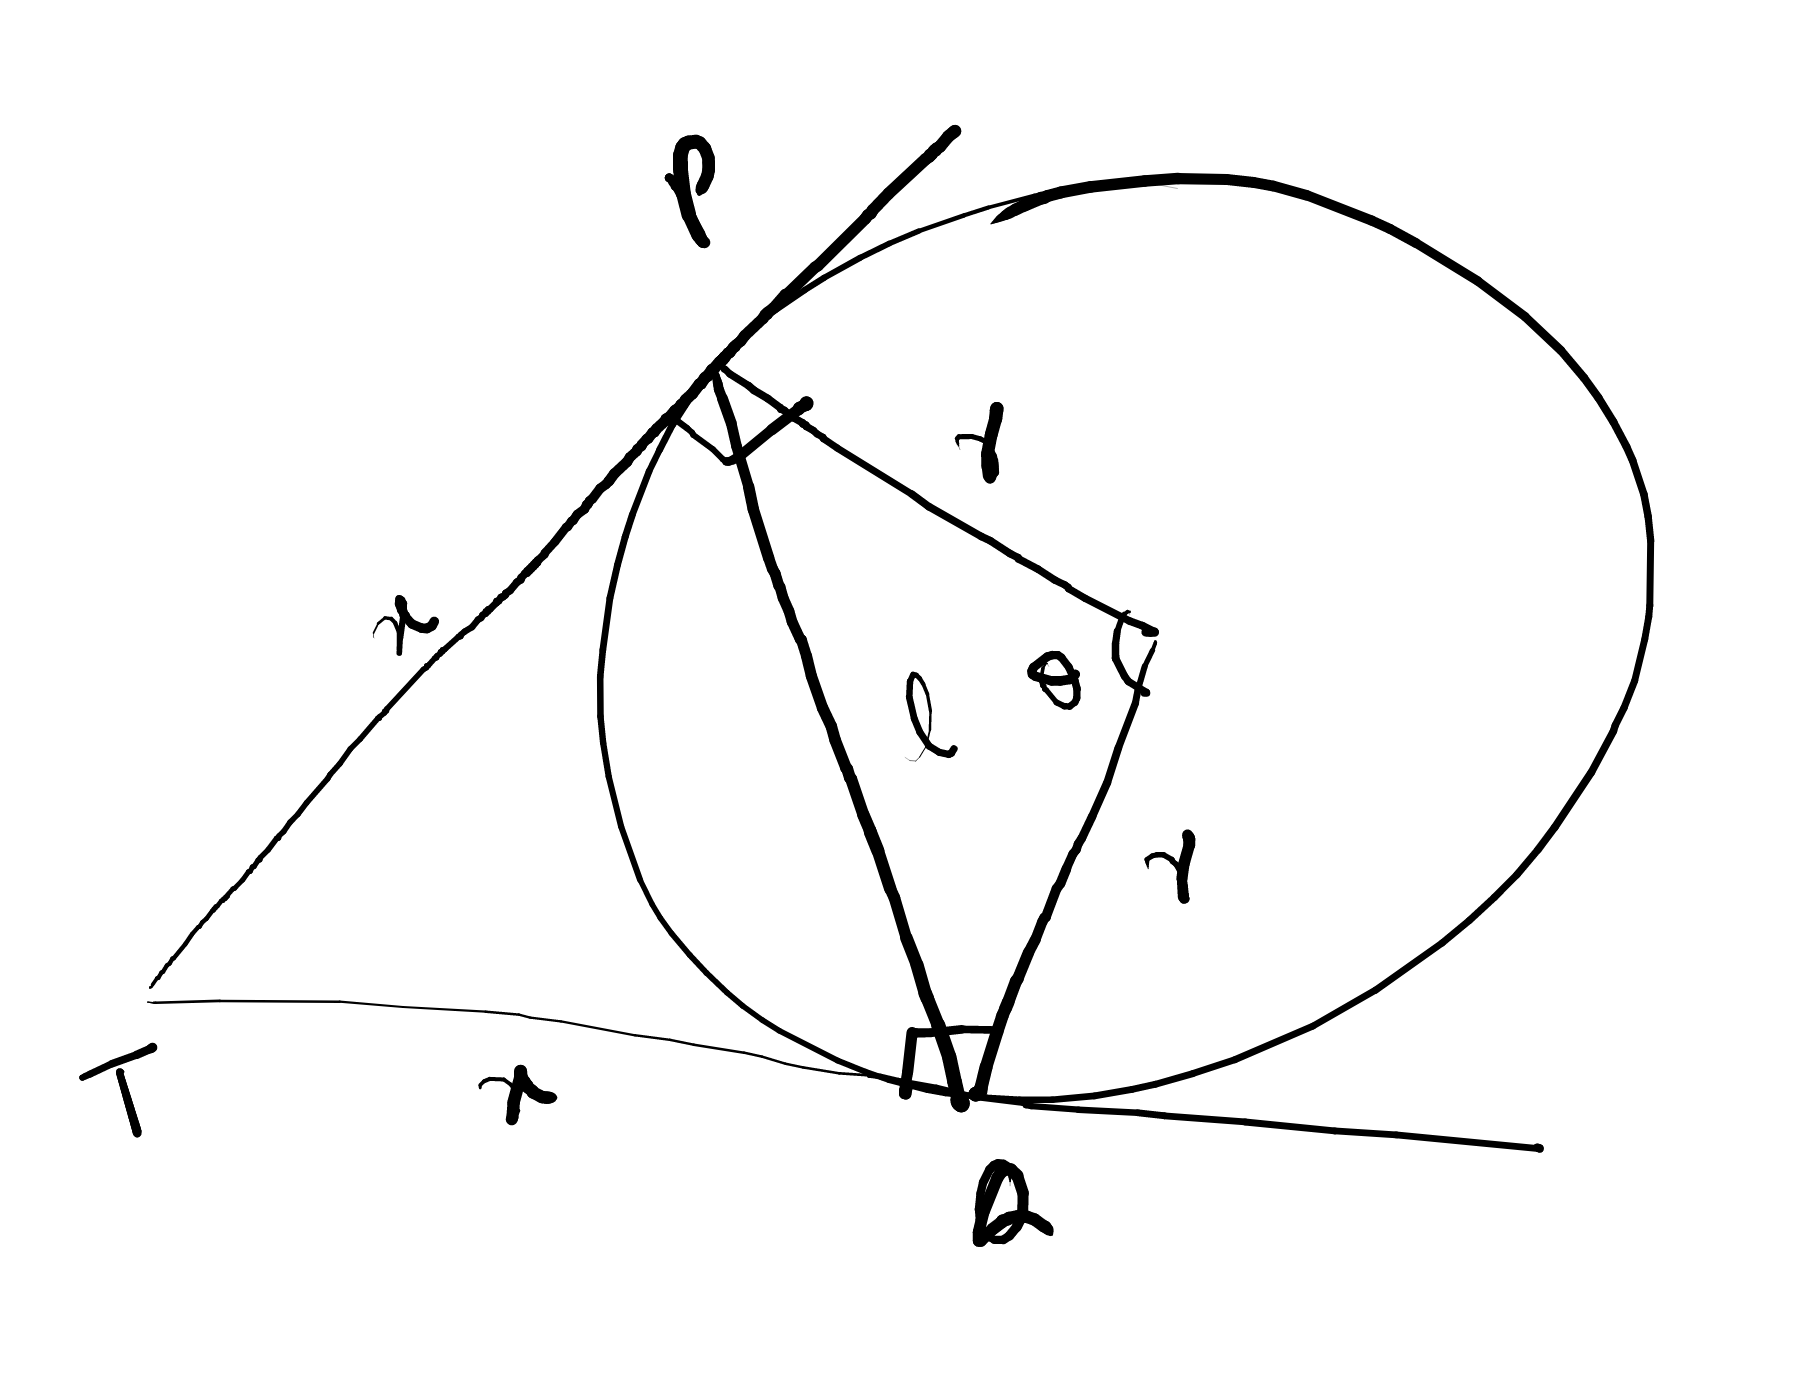
\includegraphics[width=0.6\columnwidth]{figs/ncert/circle/8.png}}
	\end{center}
	\caption{}
	\label{fig:ncert-circ-8}	
\end{figure}
%
     	\item If a circle is inscribed in a right angled triangle $ABC$ right angled at $\vec{B}$, show that the diameter of the circle is equal to $AB+BC-AC$.
\\
\solution
	In \figref{fig:ncert-circ-9}, 
\begin{align}
	a = r\brak{\cot\frac{B}{2}+\cot\frac{C}{2}} 
	\\
	b = r\brak{\cot\frac{C}{2}+\cot\frac{A}{2}} 
	\\
	c = r\brak{\cot\frac{A}{2}+\cot\frac{B}{2}} 
	\\
	\implies c+a-b = 2r\cot\frac{B}{2} = 2r\quad \because B = 90\degree
\end{align}
\begin{figure}[H]
	\begin{center}
		{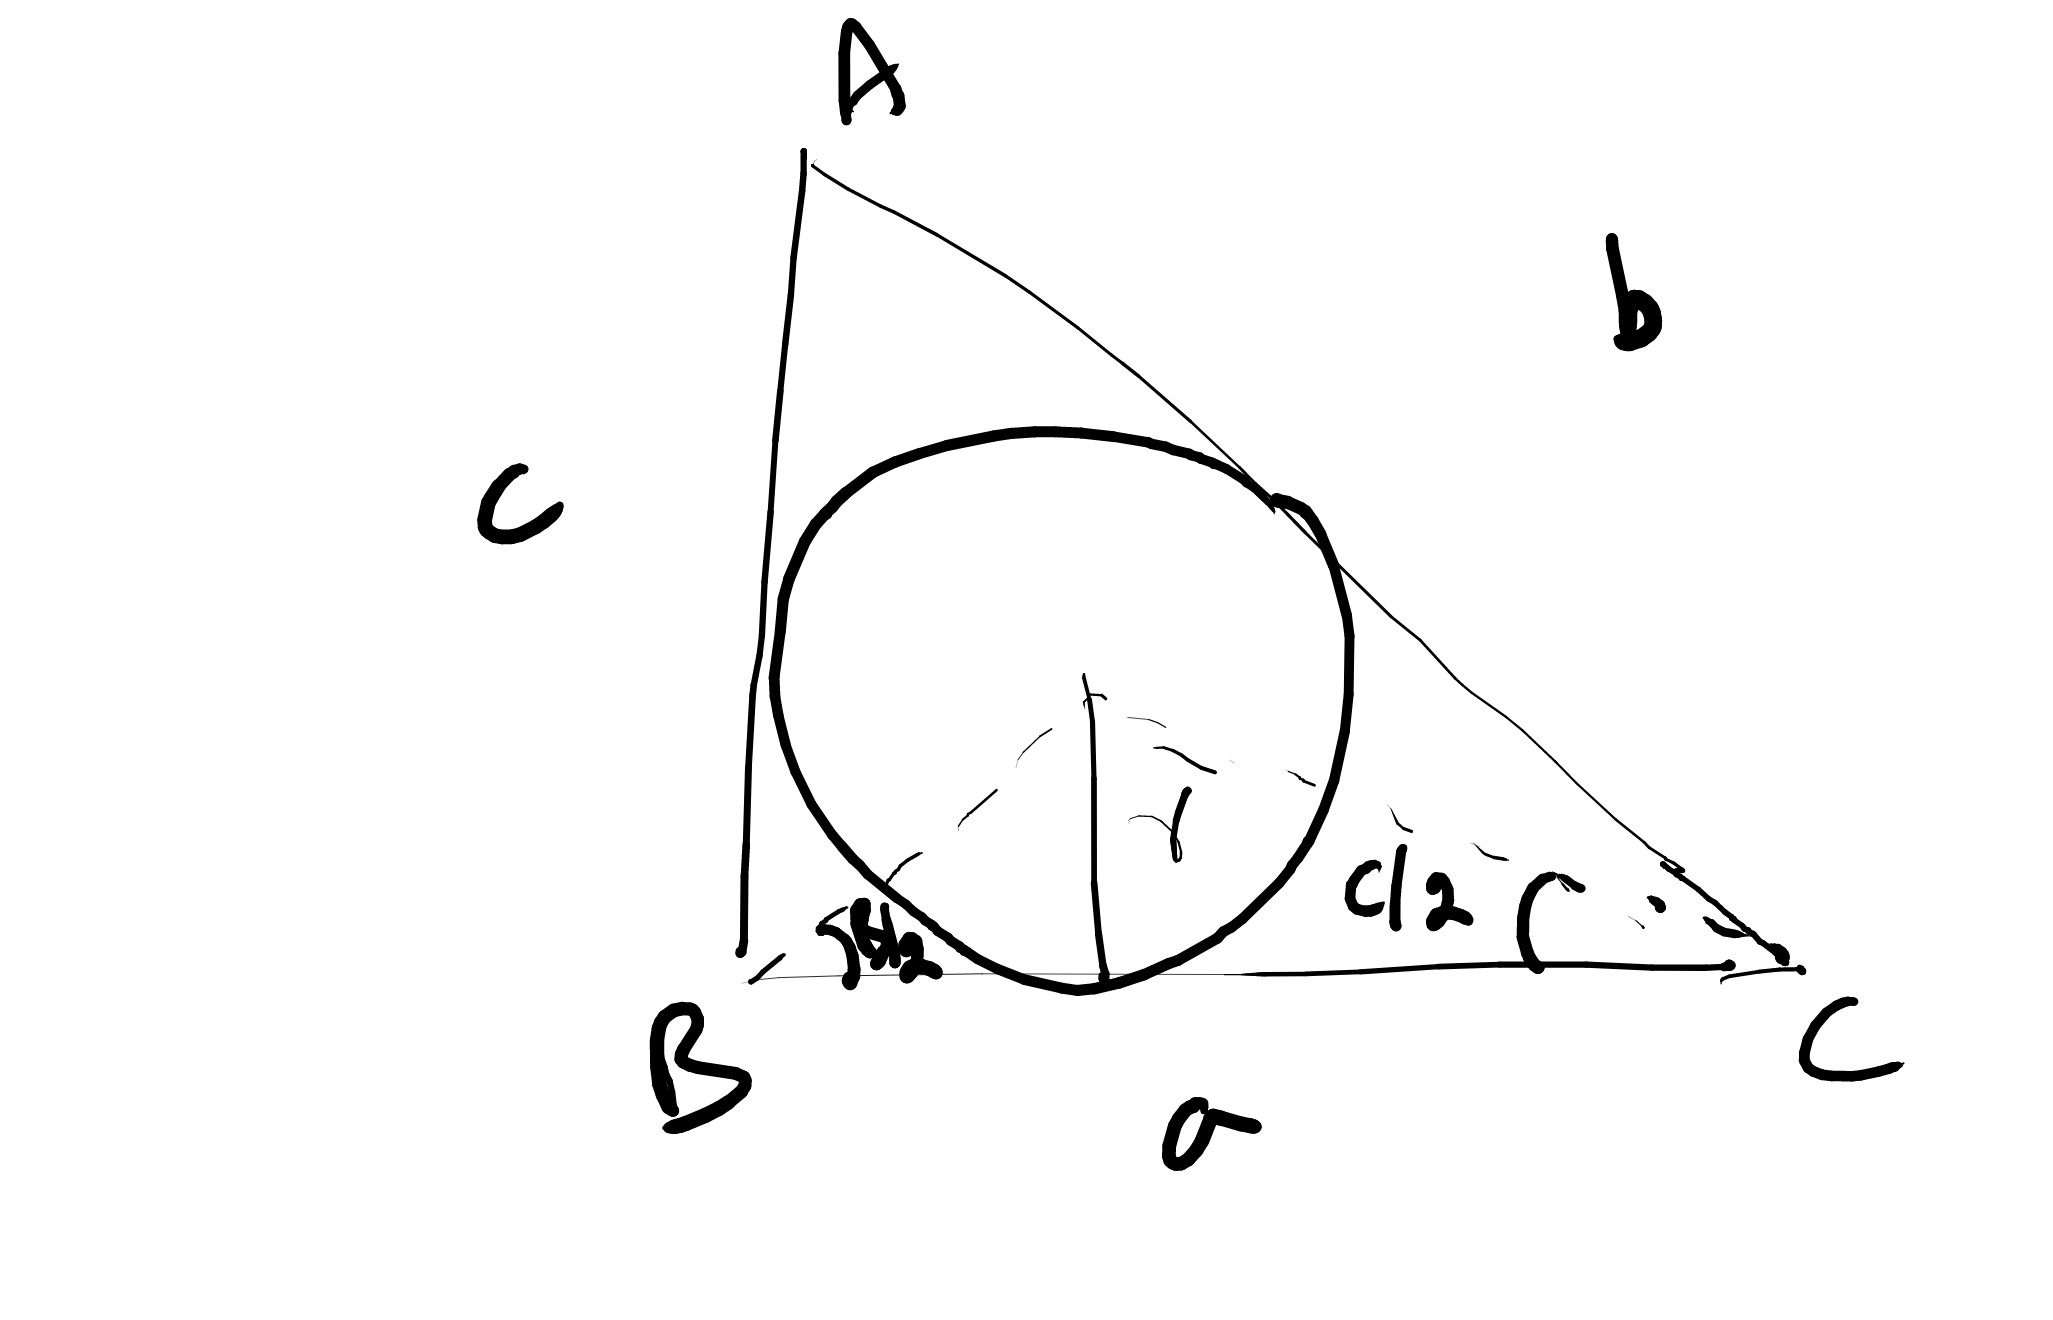
\includegraphics[width=0.6\columnwidth]{figs/ncert/circle/9.png}}
	\end{center}
	\caption{}
	\label{fig:ncert-circ-9}	
\end{figure}
\end{enumerate}
